%# -*- coding: utf-8-unix -*-

\raggedbottom
\chapter{基础算法与优化思路}
\label{chap:algorithm}

\section{引言}
经典的非交互式差分隐私匿名算法DiffGen是本课题优化算法设计的基础。本章节针对课题相关的技术对DiffGen进行介绍分析,并揭示其缺陷——在较高查询维度的请求中,DiffGen模型的本质和前文论述的频率矩阵加噪模型是一样的。接下来论述针对一维无归属直方图使用的基于一致性约束的优化技术,总结其应用特性同样适用于面向分类应用的范围计数查询需求。这也给频率矩阵模型问题提供了解决方案,并结合DiffGen算法,为接下来的优化算法做铺垫。

\section{DiffGen算法}

DiffGen算法是由Mohammed等人于2011年提出的一个非交互式差分隐私匿名算法\cite{DiffGen},基于分类树结构和指数机制构建重匿名数据集,其性能优于SuLQ-basedID3和DiffP-C4.5,但仍存在着不足。
本节的示例均基于例\ref{chap3_exmp}的背景,表述如下:
\begin{exmp}
	\label{chap3_exmp}
	某公司有8位应聘者,对“国籍”、“年龄”以及是否被录用统计如表\ref{chap3_table}(a),类属性为“是否被录用”。
\end{exmp}

\begin{table}[!hpb]
	\label{chap3_table}
	\centering
		\bicaption[tab:firstone]{表}{应聘者统计表}{Table}{The statistical table for candidates}
	\subtable[统计表]{
		\begin{tabular}{|c|c|c|}
			\hline
			$\textbf{国籍}$ & $\textbf{年龄}$ & $\textbf{是否被录用}$ \\
			\hline
			中国 & 18 & 否 \\
			\hline
			蒙古 & 21 & 是 \\
			\hline
			伊朗 & 27 & 否 \\
			\hline
			以色列 & 35 & 否 \\
			\hline
			以色列 & 29 & 是 \\
			\hline
			中国 & 39 & 是 \\
			\hline
			蒙古 & 22 & 否 \\
			\hline
			中国 & 28 & 否 \\
			\hline
		\end{tabular}}
		\qquad
		\subtable[泛化处理后的统计表]{%
			\begin{tabular}{|c|c|c|}
				\hline
				$\textbf{国籍}$ & $\textbf{年龄}$ & $\textbf{类属性计数(录用分布)}$ \\
				\hline
				东亚 & [15-25) & 3 (1是2否) \\
				\hline
				东亚 & [25-40) & 2 (1是1否) \\
				\hline
				西亚 & [15-25) & 0 (0是0否) \\
				\hline
				西亚 & [25-40) & 3 (1是2否) \\
				\hline
			\end{tabular}}
		\end{table}

\subsection{泛化技术}

泛化技术是匿名算法实现的关键技术,在DiffGen中通过匿名树(Taxonomy tree)来组织每个属性的匿名关系。如图\ref{fig:taxonomy}所示,通过指定更一般的泛化域(Dom),原属性作为叶节点,自底向上地构建匿名树。对于离散属性“国籍”,采取抽象共性的方式进行逐层泛化;对于连续属性“年龄”,通过更大的连续区间进行泛化。表\ref{chap3_table}(b)是泛化处理后的统计结果。
从根节点自顶向下来看,匿名树定义了一套划分规则(Partition guidelines),指导每个泛化属性如何分裂,如“东亚”的分裂趋势为分成“中国”和“蒙古”。显然匿名树中的属性值是不重复。

\begin{figure}[!htp]
	\centering
	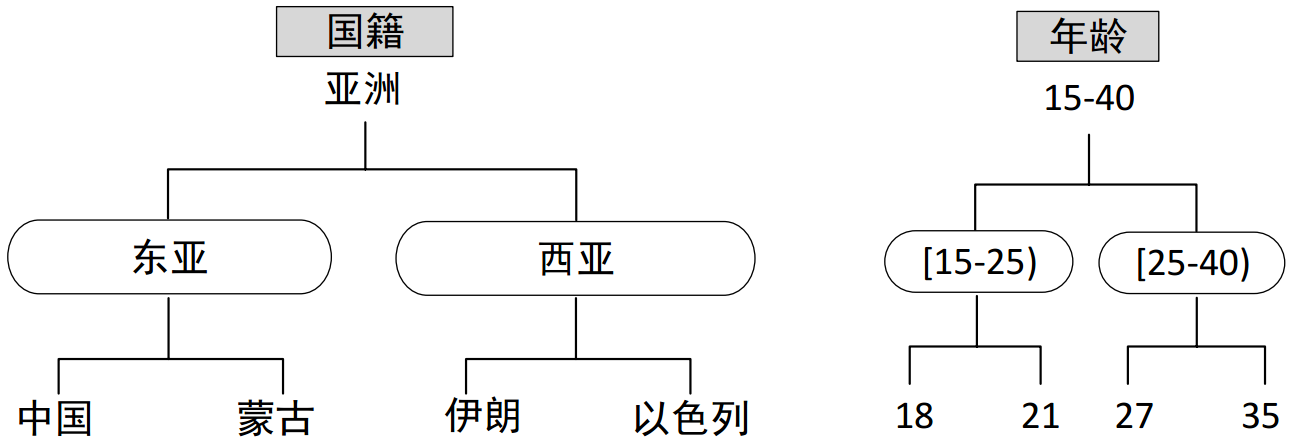
\includegraphics[width=5in]{chap3/taxonomy}
	\bicaption[fig:taxonomy]{图}{属性“国籍”和“年龄”的匿名树}{Fig.}{The taxonomy tree for 'Country' and 'Age'}
\end{figure}


\subsection{算法概述}

DiffGen算法以匿名树作为属性匿名规则,采用决策树构建的方式,在逐步构造分类树的同时对原数据集进行划分,最后发布落在叶节点的数据集。基于例\ref{chap3_exmp}的背景,结合图\ref{fig:diffgen},DiffGen算法运行过程概括如下:

\begin{figure}[!htp]
	\centering
	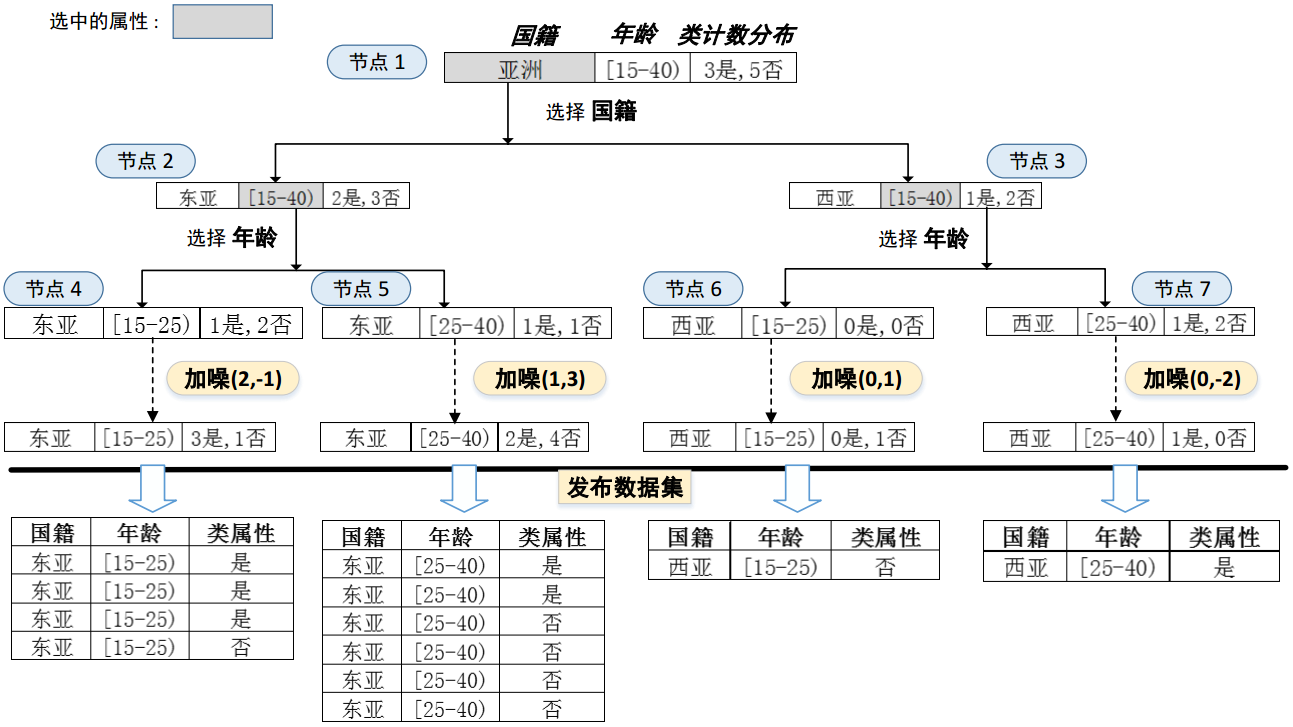
\includegraphics[width=6.2in]{chap3/diffgen}
	\bicaption[fig:diffgen]{图}{基于DiffGen算法的数据集发布流程概述}{Fig.}{The release process for dataset based DiffGen}
\end{figure}

\begin{enumerate}
	\label{process}
	\item 定义分类树高限度h。为数据集的每个属性定义匿名树结构,并组合所有匿名树的根节点属性值作为分类树的根节点条目。每个数据集条目根据属性值包含关系,归入相应的节点。例如,由各匿名树根节点属性值构成了图\ref{fig:diffgen}的节点1。对于原数据集条目\{中国,18,否\},根据各匿名树结构,显然“中国”$\in$“亚洲”,“18”$\in$“[15-40]”,因此它归入节点1。各数据条目与节点的归并关系均如此。
	\item 基于决策树构建算法,通过指数机制选取分裂属性,但与普通决策树算法不同的是,在处理连续属性和使用指数机制时引入噪音干扰以满足差分隐私定义。分裂属性的同时伴随着数据集的划分。例如,图\ref{fig:diffgen}的节点1选出属性“国籍”,根据匿名树划分为“东亚”和“西亚”,于是生成节点2和节点3,同时节点1上的数据条目也归入相应的节点上(通过类计数分布可以看出)。
	\item 重复第二步过程,直到达到迭代上限,即树高h,或者达到某属性匿名树的最“细”划分限度。如图\ref{fig:taxonomy}的椭圆气泡层即为匿名树的划分极限。
	\item 图\ref{fig:diffgen}以中间的粗直线为界,上半部分为完整的分类树,下半部分为本课题归纳的数据发布过程。DiffGen算法往分类树每个叶节点的每一类计数分布上添加拉普拉斯噪音,最后发布统计情况。发布的新数据集如表\ref{chap3_table2}。
\end{enumerate}

\begin{table}[!hpb]
	\label{chap3_table2}
	\centering
	\bicaption[tab:firstone]{表}{DiffGen算法处理后的发布数据集}{Table}{The realesed dataset after DiffGen}
	\subtable[数据项1]{
		\begin{tabular}{|c|c|c|}
			\hline
			$\textbf{国籍}$ & $\textbf{年龄}$ & $\textbf{是否被录用}$ \\
			\hline
			东亚 & [15-25) & 是 \\
			\hline
			东亚 & [15-25) & 是 \\
			\hline
			东亚 & [15-25) & 是 \\
			\hline
			东亚 & [15-25) & 否 \\
			\hline
		\end{tabular}}
		\qquad
		\subtable[数据项2]{%
		\begin{tabular}{|c|c|c|}
			\hline
			$\textbf{国籍}$ & $\textbf{年龄}$ & $\textbf{是否被录用}$ \\
			\hline
			东亚 & [25-40) & 是 \\
			\hline
			东亚 & [25-40) & 是 \\
			\hline
			东亚 & [25-40) & 否 \\
			\hline
			东亚 & [25-40) & 否 \\
			\hline
			东亚 & [25-40) & 否 \\
			\hline
			东亚 & [25-40) & 否 \\
			\hline
		\end{tabular}}
		\qquad
		\subtable[数据项3]{%
		\begin{tabular}{|c|c|c|}
			\hline
			$\textbf{国籍}$ & $\textbf{年龄}$ & $\textbf{是否被录用}$ \\
			\hline
			西亚 & [15-25) & 否 \\
			\hline
		\end{tabular}}
		\qquad
		\subtable[数据项4]{%
		\begin{tabular}{|c|c|c|}
			\hline
			$\textbf{国籍}$ & $\textbf{年龄}$ & $\textbf{是否被录用}$ \\
			\hline
			西亚 & [25-40) & 是 \\
			\hline
		\end{tabular}}
\end{table}


\subsection{算法缺陷探讨}

图\ref{fig:diffgen}的下半部分对流程\ref{process}的第四步进行展开,归纳了DiffGen算法的数据发布过程。根据分类树的构建方法,每个叶节点中的数据项拥有相同的属性值,区别仅在于类计数分布上。组织所有叶节点上的数据项,可以看出这其实就是一个频率矩阵。那么,DiffGen往叶节点的每个类分布加噪的方式其实就等同于往频率矩阵的每个行项加噪。每个叶节点数据集的属性值组合构成了当前叶节点的属性值集合,如节点4的代表的集合为\{东亚,[15-25]\}。很显然,每个叶节点所代表的集合是两两不相交的,例如在除了节点4以外的叶节点中必然不存在集合\{东亚,[15-25]\}。可通过简单的反证法证明。
\begin{prop}
 	\label{prop1}
 DiffGen分类树中,每个叶节点的属性值构成的集合是两两不相交的。	
\end{prop}
 
\begin{proof}
  假设命题\ref{prop1}为假,即在DiffGen分类树中,存在两个相交的叶节点,也就是对于某一属性值集合为\{a,b,c\}的叶节点A,存在另一属性值集合为\{a,b,c\}的叶节点B,且A,B不为同一节点。
  	
  根据分类树,寻找A,B的最小公共祖先节点C,得到节点C的分裂属性Ca及Ca的匿名树。由于A与B相交,显然Ca的匿名树在Ca上的划分产生了两个一样的属性值x,x$\in$\{a,b,c\}。具有重复属性值x的结论与匿名树的定义矛盾。因此,命题\ref{prop1}为真。
\end{proof}

命题\ref{prop1}的成立也意味着DiffGen的叶节点集满足差分隐私的水平组合性质\cite{dpcombination},即叶节点上拉普拉斯噪音的敏感性为一常量,每个叶节点的加噪和应答是相互独立的。例如,在发布数据集上运行决策树分类算法,计算总熵值时需要对全属性分布的计数情况进行累加计算,此时含噪的[数据项1,2,3,4]线性叠加;当计算“东亚”的熵值时,需要[数据项1,2]的线性叠加运算。
可以看到,问题又回到了以行项为单位的独立加噪和处理模式上。因此,在范围查询需求的应用中,DiffGen模型的本质和前文所讨论的频率矩阵加噪模型是一致的,噪音的线性叠加问题制约者发布数据的可用性。


\section{一致性特性}

\subsection{无归属直方图的一致性约束优化}


\subsection{框架适用性探讨}